\chapter{Results}
In the next section two error metrics are briefly described, followed by evaluations of each experiment. At the beginning of each section a small description of the problem setting is given, followed by the results and discussion.

\section{Error Metrics}
For this thesis two error metrics were considered:
\begin{itemize}
  \item \textbf{Point Distance:} Given two meshes with equal topology, meaning both meshes have the same amount of vertices and layout, the error computed is based on the distance between corresponding points. In general, the mean distance is computed over all point correspondences.
  \item \textbf{Face orientations:} The idea behind this method is based on the $\mathbf{Q}$ matrix mentioned in section \ref{faceDeform}. Given two topologically equal meshes, the $\mathbf{Q}$ matrix is computed for all corresponding faces. As it is of interest to investigate the difference in breast shapes, this error tries to quantify the variation of the $\mathbf{Q}$ matrices.
\end{itemize}

One drawback of the point distance method occurs when the two meshes are not aligned properly. This can be solved by applying the same algorithm mentioned in section \ref{align} before computing the error. One advantage of this method is the unit of the error, as it could be converted into a unit of distance, given the distance between two point is known in real world lengths. This error can also be computed when two meshes are not topologically equal by first finding the correspondences between vertices.\\
One advantage of the face orientation method is the invariance of translation and global rotation. This means that moving or rotating the mesh doesn't affect the error. On the other hand, the values of this error don't have a real world meaning and it is a lot harder to apply this method to topologically different meshes, as finding correspondences between faces is a lot more challenging.\\
The methods are depicted in figure \ref{fig:errordiag}. Both methods have their advantages and disadvantages, but due to the fact that alignment isn't a problem, the error metric used in this thesis is the point distance method.

\begin{figure}
\centering
\begin{subfigure}{.5\textwidth}
  \centering
  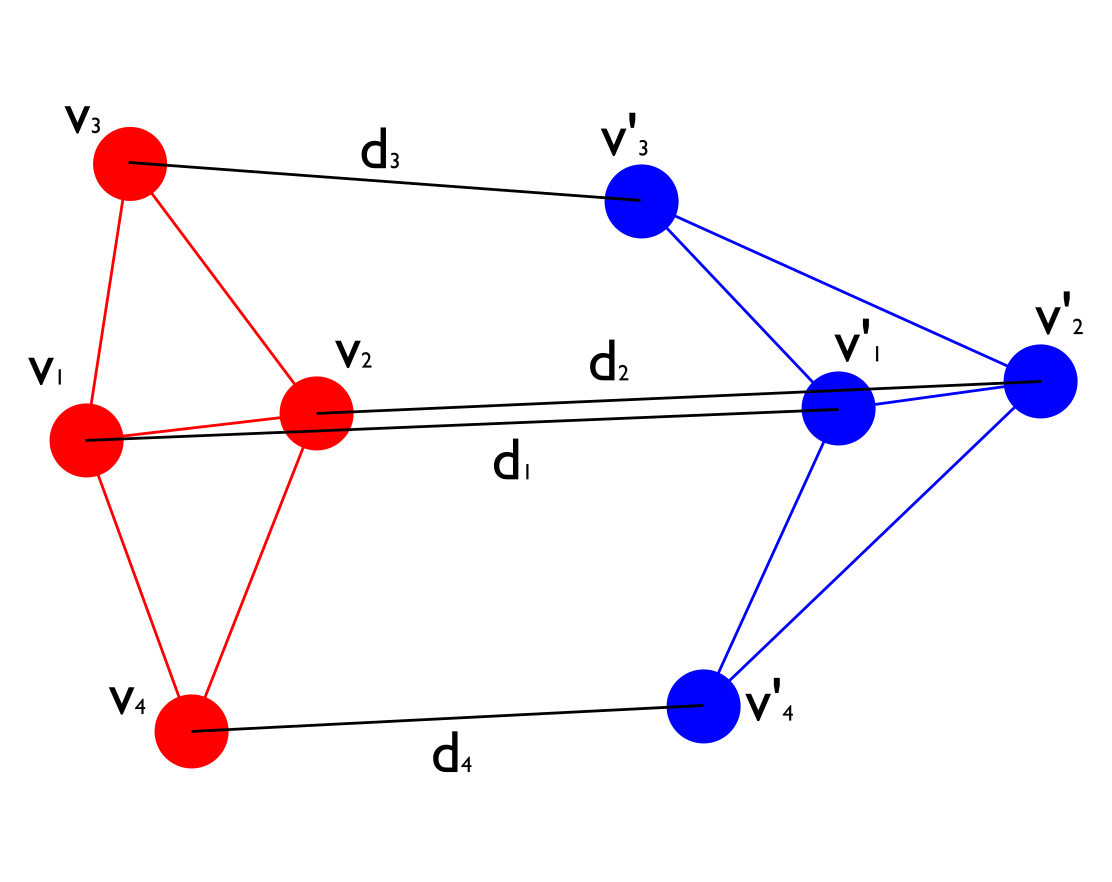
\includegraphics[width=.75\linewidth]{figures/pediag}
\end{subfigure}%
\begin{subfigure}{.5\textwidth}
  \centering
  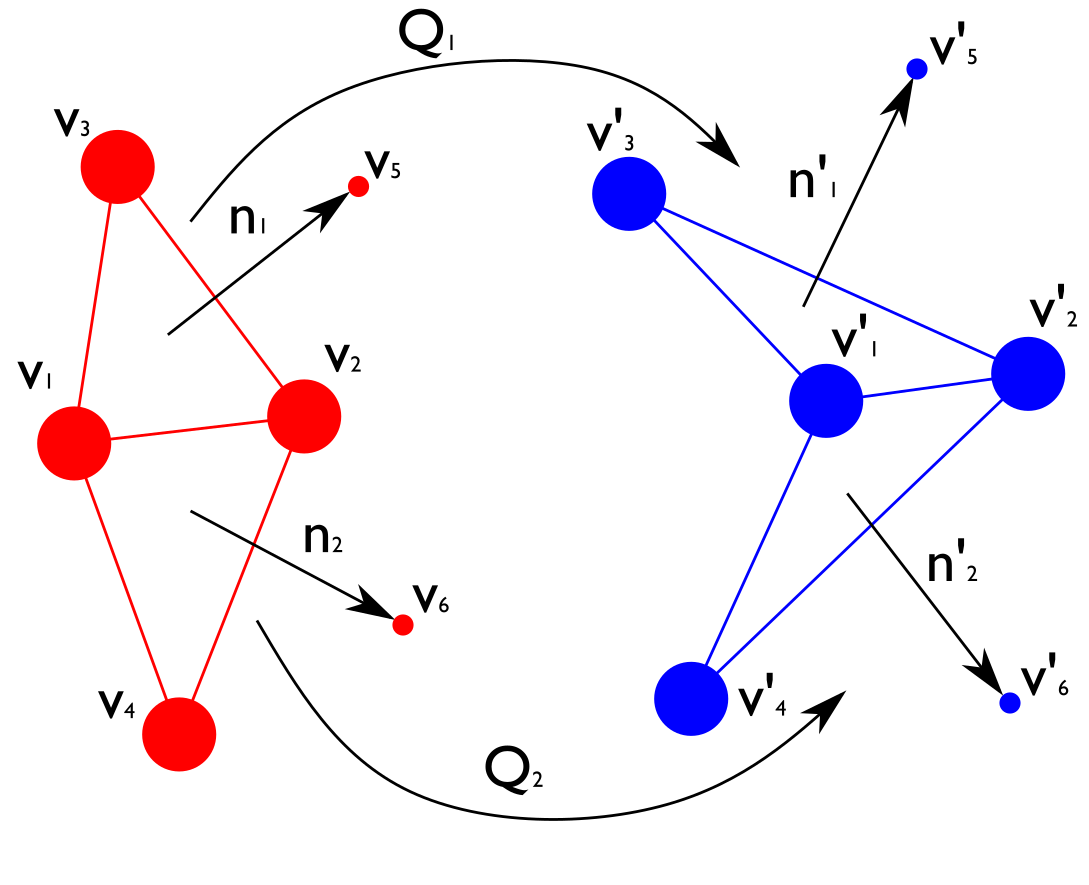
\includegraphics[width=.75\linewidth]{figures/dediag}
\end{subfigure}
\caption{The left image depicts distances between corresponding points of the mesh. The right image shows a representation of the information used to compute the $\mathbf{Q}$ matrix.}
\label{fig:errordiag}
\end{figure}

\section{Evaluation}

\subsection{Mesh Point Error} % Compare to GT

\subsection{Fit to Pointcloud} % Compare to NRICP vs Ceres

\section{PCA point/normals/deform}

\section{Learning mapping}

\section{Data MH vs NRICP}

\section{Data Real vs NRICP}

\chapter{Conclusion and Outlook}
